\documentclass[11pt,a4paper]{article}

% =============================================================================
% CONFIGURACIÓN DE PAQUETES Y ESTILO ACADÉMICO
% =============================================================================
\usepackage[utf8]{inputenc}
\usepackage[spanish,es-tabla]{babel}
\usepackage[margin=2.0cm,top=2.2cm,bottom=2.2cm]{geometry}
\usepackage{graphicx}
\usepackage{subcaption}
\usepackage{booktabs}
\usepackage{tabularx}
\usepackage{amsmath}
\usepackage{amssymb}
\usepackage{amsfonts}
\usepackage{xcolor}
\usepackage{fancyhdr}
\usepackage{titlesec}
\usepackage{listings}
\usepackage{microtype}
\usepackage{hyperref}

% Definición de colores institucionales y de código
\definecolor{uaBlue}{RGB}{20, 50, 110}
\definecolor{uaDarkSlate}{RGB}{35, 45, 60}
\definecolor{codeBg}{RGB}{248, 249, 250}
\definecolor{codeFrame}{RGB}{220, 224, 230}
\definecolor{codeGreen}{RGB}{46, 139, 87}
\definecolor{codePurple}{RGB}{128, 0, 128}

% Configuración de hipervínculos
\hypersetup{
    colorlinks=true,
    linkcolor=uaBlue,
    citecolor=uaBlue,
    urlcolor=uaBlue,
    pdftitle={Memoria Técnica - Práctica 1: Robótica Móvil y Manipulación},
    pdfauthor={Santiago Álvarez Geanta, Guillermo García Blázquez, David Martínez Gómez, Taron Sargsyan}
}

% Configuración de cabeceras y pies de página
\pagestyle{fancy}
\fancyhf{}
\fancyhead[L]{\small\textcolor{uaDarkSlate}{\textbf{Robótica Inteligente} \textbar\ Práctica 1}}
\fancyhead[R]{\small\textcolor{uaDarkSlate}{EPS \textbar\ Universidad de Alicante}}
\fancyfoot[C]{\thepage}
\renewcommand{\headrulewidth}{0.6pt}
\renewcommand{\footrulewidth}{0.3pt}

% Formato de títulos de sección
\titleformat{\section}{\color{uaBlue}\normalfont\Large\bfseries}{\thesection}{1em}{}[\titlerule]
\titleformat{\subsection}{\color{uaDarkSlate}\normalfont\large\bfseries}{\thesubsection}{1em}{}
\titleformat{\subsubsection}{\color{uaDarkSlate}\normalfont\normalsize\bfseries}{\thesubsubsection}{1em}{}

% Configuración de listados de código
\lstset{
    backgroundcolor=\color{codeBg},
    basicstyle=\ttfamily\footnotesize,
    breaklines=true,
    frame=single,
    rulecolor=\color{codeFrame},
    numbers=none,
    keywordstyle=\color{uaBlue}\bfseries,
    commentstyle=\color{codeGreen}\itshape,
    stringstyle=\color{codePurple},
    showstringspaces=false,
    tabsize=2,
    aboveskip=5pt,
    belowskip=5pt
}

\setlength{\textfloatsep}{10pt plus 2pt minus 2pt}
\setlength{\intextsep}{8pt plus 2pt minus 2pt}

\graphicspath{{capturas/bloque2/}{capturas/bloque4/}{../diagramas/}{diagramas/}}

% =============================================================================
% INICIO DEL DOCUMENTO
% =============================================================================
\begin{document}

\hypersetup{pageanchor=false}
\begin{titlepage}
    \centering
    \vspace*{1.0cm}
    {\Huge\bfseries\color{uaBlue} Universidad de Alicante}\\[0.3cm]
    {\LARGE\bfseries\color{uaDarkSlate} Escuela Politécnica Superior}\\[0.2cm]
    {\large Grado en Ingeniería en Inteligencia Artificial \textbar\ Curso 4º (2026/2027)}\\[1.8cm]

    \rule{\linewidth}{1.5pt}\\[0.4cm]
    {\huge\bfseries\color{uaBlue} Robótica Inteligente (33683)}\\[0.3cm]
    {\Large\bfseries Memoria Técnica de Práctica 1}\\[0.2cm]
    {\large\itshape Introducción a las Herramientas Básicas para Robótica Móvil y Manipulación:\\
    ROS 2, Gazebo Harmonic, Nav2, MoveIt 2 y Oxford Spires Dataset}\\[0.3cm]
    \rule{\linewidth}{1.5pt}\\[1.4cm]

    \begin{minipage}{0.48\textwidth}
        \begin{flushleft}
            \textbf{\color{uaBlue} Profesor / Tutor:}\\[0.15cm]
            M.A. Muñoz-Bañón\\
            \small Dpto. de Física, Ingeniería de Sistemas\\
            y Teoría de la Señal\\[0.6cm]
            \textbf{\color{uaBlue} Fecha de Evaluación:}\\[0.15cm]
            Octubre de 2026
        \end{flushleft}
    \end{minipage}
    \hfill
    \begin{minipage}{0.48\textwidth}
        \begin{flushright}
            \textbf{\color{uaBlue} Equipo de Prácticas:}\\[0.15cm]
            Santiago Álvarez Geanta\\
            Guillermo García Blázquez\\
            David Martínez Gómez\\
            Taron Sargsyan
        \end{flushright}
    \end{minipage}

    \vfill
    {\small Entorno de ejecución: ROS 2 Jazzy Jalisco \textbar\ Gazebo Harmonic 8.0 \textbar\ Ubuntu 24.04 LTS (Docker)}
\end{titlepage}
\hypersetup{pageanchor=true}

\newpage
\pagenumbering{roman}
\tableofcontents
\newpage
\pagenumbering{arabic}

% ---------------------------
% 1. INTRODUCCIÓN GENERAL DE LA PRÁCTICA
% ---------------------------
\section{Introducción y Estructura Global de la Práctica}

La presente memoria técnica documenta el desarrollo y análisis experimental de la \textbf{Práctica 1 de Robótica Inteligente}. El objetivo consiste en adquirir destreza práctica en las herramientas estándar de robótica: el middleware \textbf{ROS 2 (Jazzy Jalisco)}, el simulador \textbf{Gazebo Harmonic}, la pila de navegación autónoma \textbf{Nav2}, la odometría LiDAR-inercial (\textbf{RKO-LIO}) y la manipulación robótica con \textbf{MoveIt 2}.

El desarrollo se realiza sobre el contenedor \textbf{Docker} oficial de la asignatura, configurado con soporte para aceleración gráfica y visualización mediante X11, lo que garantiza un entorno reproducible y aislado.

\subsection{Estructura Modular de la Práctica}
De acuerdo con las directrices de la guía docente, la práctica se estructura en cuatro bloques secuenciales:
\begin{itemize}
    \item \textbf{Bloque 1 -- Fundamentos de ROS 2:} Dominio de la arquitectura orientada a grafos de nodos, canales asíncronos (tópicos), llamadas síncronas (servicios) y tareas continuas con retroalimentación (acciones).
    \item \textbf{Bloque 2 -- Mapeo y Navegación Autónoma (Nav2):} Generación de mapas de ocupación 2D mediante SLAM, localización probabilística con filtros de partículas (AMCL) y control de plataforma móvil diferencial \textit{TurtleBot 4} empleando la pila \textit{Nav2}.
    \item \textbf{Bloque 3 -- Odometría LiDAR-Inercial (LIO) con Datos Reales:} Procesamiento sensorial denso sobre secuencias reales del \textit{Oxford Spires Dataset} (Keble College) mediante el pipeline \textit{RKO-LIO}.
    \item \textbf{Bloque 4 -- Manipulación Robótica (MoveIt 2):} Control cinemático cartesiano y articular del brazo industrial \textit{Universal Robots UR3e} (6 DOF) en simulación dinámica y planificación libre de colisiones.
\end{itemize}

\vspace{1em}

% ---------------------------
% 2. DESARROLLO DEL BLOQUE 2: MAPEO Y NAVEGACIÓN AUTÓNOMA (TURTLEBOT 4 + NAV2)
% ---------------------------
\section{Bloque 2 -- Mapeo y Navegación Autónoma con TurtleBot 4 y Nav2}

\subsection{Contexto y Plataforma Móvil Diferencial}

En este bloque se aborda la configuración y evaluación práctica de la navegación autónoma con el TurtleBot 4: generación del mapa del entorno con SLAM, estimación de la posición con el filtro de partículas AMCL y desplazamiento reactivo hacia metas mediante Nav2.

La plataforma utilizada es el \textbf{TurtleBot 4}, un robot móvil de tracción diferencial estándar en investigación educativa que integra:
\begin{itemize}
    \item \textbf{Base motriz diferencial (iRobot Create 3):} Dos ruedas motrices independientes y dos ruedas locas de apoyo, equipada con encoders ópticos en cada rueda para el cálculo de la odometría cinemática y sensores de contacto (\textit{bumpers}).
    \item \textbf{Sensor LiDAR 2D (RPLIDAR):} Escáner láser montado en la parte superior del chasis que proporciona barridos de 360 grados en el plano horizontal a través del tópico \texttt{/scan}, permitiendo detectar paredes y obstáculos en un radio de hasta 12 metros.
    \item \textbf{Cámara RGB-D estéreo (OAK-D-PRO):} Módulo de visión espacial para percepción de profundidad tridimensional.
\end{itemize}

Todo el sistema opera simulado en \textbf{Gazebo Harmonic}, sincronizado mediante el reloj de simulación de ROS 2 (\texttt{/clock}) y coordinado a través del middleware ROS 2 Jazzy.

\subsection{Mapeo del Entorno con SLAM y Teleoperación}

Para que un robot navegue de forma global, necesita conocer previamente la geometría del espacio. Dado que partimos de un entorno desconocido, recurrimos al paradigma \textbf{SLAM} (\textit{Simultaneous Localization and Mapping}), donde el robot estima simultáneamente su propia trayectoria y construye el mapa del entorno.

\subsubsection{Despliegue y Exploración Manual}
El proceso de mapeo se estructuró en los siguientes pasos:
\begin{enumerate}
    \item \textbf{Arranque del simulador:} Se cargó el mundo virtual de laboratorio con el TurtleBot 4 mediante:
\begin{lstlisting}[language=bash]
ros2 launch turtlebot4_gz_bringup turtlebot4_gz.launch.py model:=standard rviz2:=false
\end{lstlisting}
    \item \textbf{Lanzamiento del algoritmo SLAM:} Se ejecutó el nodo de mapeo (\texttt{slam\_toolbox} / Cartographer):
\begin{lstlisting}[language=bash]
ros2 launch turtlebot4_navigation slam.launch.py
\end{lstlisting}
    \item \textbf{Teleoperación por teclado:} Para cubrir todas las estanterías y pasillos del laboratorio, se utilizó el nodo \texttt{teleop\_twist\_keyboard}, enviando comandos de velocidad angular y lineal (\texttt{TwistStamped}) a través de la interfaz de control:
\begin{lstlisting}[language=bash]
ros2 run teleop_twist_keyboard teleop_twist_keyboard --ros-args -r /cmd_vel:=/cmd_vel_unstamped
\end{lstlisting}
    \item \textbf{Almacenamiento del mapa:} Una vez recorrido todo el entorno y cerrado el lazo del mapa en RViz2, se exportó la rejilla de ocupación 2D generada mediante la herramienta \texttt{nav2\_map\_server}:
\begin{lstlisting}[language=bash]
ros2 run nav2_map_server map_saver_cli -f /home/developer/ros2_ws/mapa_laboratorio
\end{lstlisting}
    Este comando produjo dos ficheros: \texttt{mapa\_laboratorio.pgm} (imagen rasterizada en escala de grises donde el negro representa obstáculos, el blanco espacio libre y el gris celdas desconocidas) y \texttt{mapa\_laboratorio.yaml} (metadatos con resolución de 0.03\,m/celda y punto de origen).
\end{enumerate}

\begin{figure}[htbp]
    \centering
    \begin{subfigure}[b]{0.32\textwidth}
        \centering
        \includegraphics[width=\textwidth]{b2_01_gazebo.png}
        \caption{TurtleBot 4 en Gazebo Harmonic.}
        \label{fig:b2_gazebo}
    \end{subfigure}
    \hfill
    \begin{subfigure}[b]{0.32\textwidth}
        \centering
        \includegraphics[width=\textwidth]{b2_02_slam.png}
        \caption{Lanzamiento del nodo SLAM.}
        \label{fig:b2_slam_node}
    \end{subfigure}
    \hfill
    \begin{subfigure}[b]{0.32\textwidth}
        \centering
        \includegraphics[width=\textwidth]{b2_03_rviz_slam.png}
        \caption{Construcción del mapa en RViz2.}
        \label{fig:b2_rviz_slam}
    \end{subfigure}
    \\[6pt]
    \begin{subfigure}[b]{0.48\textwidth}
        \centering
        \includegraphics[width=\textwidth]{b2_04_teleop.png}
        \caption{Teleoperación manual con teclado.}
        \label{fig:b2_teleop}
    \end{subfigure}
    \hfill
    \begin{subfigure}[b]{0.48\textwidth}
        \centering
        \includegraphics[width=\textwidth]{b2_05_slam_dual.png}
        \caption{Inspección combinada Gazebo + RViz2 durante el mapeo.}
        \label{fig:b2_slam_dual}
    \end{subfigure}
    \caption{Secuencia experimental completa de la fase de Mapeo (SLAM): despliegue en simulación, exploración guiada por teleoperación y generación de la rejilla de ocupación 2D.}
    \label{fig:grid_slam}
\end{figure}

\subsection{Localización Basada en Mapa con Filtro de Partículas (AMCL)}

Una vez generado el mapa estático, el robot ya no necesita calcular SLAM (proceso computacionalmente costoso), sino que pasa a utilizar el algoritmo \textbf{AMCL} (\textit{Adaptive Monte Carlo Localization}).

AMCL es un filtro de partículas que estima la posición y orientación del robot $(x, y, \theta)$ en el mapa comparando en tiempo real las lecturas del escáner láser (\texttt{/scan}) con las paredes y obstáculos de la rejilla de ocupación:
\begin{enumerate}
    \item \textbf{Carga del mapa (\texttt{map\_server}):} El nodo \texttt{map\_server} publica el mapa estático en el tópico \texttt{/map} con durabilidad \textit{transient local}.
    \item \textbf{Pose Inicial (\textit{2D Pose Estimate}):} Dado que el filtro de partículas necesita una hipótesis de partida, se proporciona una estimación aproximada mediante la herramienta interactiva de RViz2 (o publicando en el tópico \texttt{/initialpose}).
    \item \textbf{Convergencia de partículas:} AMCL genera una nube de hipótesis representadas mediante flechas verdes (\texttt{/particle\_cloud}). Conforme el robot recibe nuevas lecturas LiDAR y se desplaza, las partículas que coinciden con la geometría del entorno aumentan su peso probabilístico y las demás desaparecen, haciendo que la nube colapse sobre la posición real del vehículo.
    \item \textbf{Corrección de la odometría:} Con la pose estimada, AMCL publica continuamente la transformación dinámica \texttt{map -> odom}, corrigiendo en tiempo real la deriva acumulada por el deslizamiento de las ruedas en la odometría.
\end{enumerate}

\begin{figure}[htbp]
    \centering
    \begin{subfigure}[b]{0.32\textwidth}
        \centering
        \includegraphics[width=\textwidth]{b2_06_amcl_map.png}
        \caption{Lanzamiento de \texttt{map\_server} y AMCL.}
        \label{fig:b2_amcl_terminal}
    \end{subfigure}
    \hfill
    \begin{subfigure}[b]{0.32\textwidth}
        \centering
        \includegraphics[width=\textwidth]{b2_08_rviz_map.png}
        \caption{Mapa estático cargado en RViz2.}
        \label{fig:b2_rviz_map}
    \end{subfigure}
    \hfill
    \begin{subfigure}[b]{0.32\textwidth}
        \centering
        \includegraphics[width=\textwidth]{b2_09_amcl_costmap.png}
        \caption{Pose estimada y capas de \textit{costmap}.}
        \label{fig:b2_costmap_init}
    \end{subfigure}
    \caption{Fase de localización probabilística: servicio de mapas, inyección de pose inicial en RViz2 y activación de las capas de coste global.}
    \label{fig:grid_amcl}
\end{figure}

\subsection{Pila de Navegación Nav2 y Planificación de Trayectorias}

Con el robot correctamente localizado en el mapa, se activa la pila de navegación autónoma \textbf{Nav2} (\texttt{nav2.launch.py}). Nav2 se estructura en una arquitectura modular gobernada por un Árbol de Comportamiento (\textit{Behavior Tree}):

\subsubsection{Mapas de Coste (Costmaps 2D)}
Para navegar con seguridad, Nav2 mantiene dos representaciones espaciales basadas en celdas de coste (donde 0 representa espacio libre, 254 obstáculo letal y los valores intermedios zonas de precaución):
\begin{itemize}
    \item \textbf{Global Costmap:} Abarca todo el mapa del laboratorio. Integra la capa estática del mapa (\texttt{static\_layer}), la capa de obstáculos de sensores (\texttt{obstacle\_layer}) y una capa de inflado (\texttt{inflation\_layer}) que expande los límites de los obstáculos en función del radio del chasis del robot, evitando que el planificador trace rutas rozando paredes.
    \item \textbf{Local Costmap:} Una ventana móvil de dimensiones reducidas centrada en el robot. Se actualiza a alta frecuencia con los datos frescos del LiDAR para detectar obstáculos imprevistos o personas en movimiento que no aparecían en el mapa original.
\end{itemize}

\subsubsection{Planificador Global y Controlador Local}
La navegación se divide en dos niveles complementarios:
\begin{enumerate}
    \item \textbf{Planificador Global (\texttt{planner\_server}):} Emplea el plugin \textit{Navfn} (basado en el algoritmo $A^*$ / Dijkstra) sobre el \textit{Global Costmap} para calcular el camino geométrico óptimo desde la posición actual hasta el objetivo fijado.
    \item \textbf{Controlador Local (\texttt{controller\_server}):} Ejecuta el algoritmo \textit{MPPI} (\textit{Model Predictive Path Integral}) sobre el \textit{Local Costmap}. Genera miles de trayectorias candidatas en tiempo real respetando la cinemática diferencial del robot y selecciona la velocidad lineal y angular óptima, esquivando obstáculos imprevistos y publicando consignas en \texttt{/cmd\_vel}.
    \item \textbf{Navegador de Comportamientos (\texttt{bt\_navigator}):} Supervisa la ejecución global. Si el robot se queda atascado o un obstáculo bloquea el paso, activa el servidor de recuperaciones (\texttt{behavior\_server}) para retroceder (\textit{backup}) o girar sobre su eje (\textit{spin}) antes de replanificar.
\end{enumerate}

\begin{figure}[htbp]
    \centering
    \begin{subfigure}[b]{0.48\textwidth}
        \centering
        \includegraphics[width=\textwidth]{b2_07_nav2_nodes.png}
        \caption{Inicialización de servidores Nav2.}
        \label{fig:b2_nav2_terminal}
    \end{subfigure}
    \hfill
    \begin{subfigure}[b]{0.48\textwidth}
        \centering
        \includegraphics[width=\textwidth]{b2_10_goal_pose.png}
        \caption{Navegación hacia objetivo interactivo (\textit{2D Goal Pose}).}
        \label{fig:b2_goal_pose}
    \end{subfigure}
    \caption{Activación de la pila Nav2 y desplazamiento autónomo hacia una meta seleccionada interactivamente en RViz2.}
    \label{fig:grid_nav2_goal}
\end{figure}

\subsection{Introspección del Middleware ROS 2 (Sección 6.1)}

Siguiendo las indicaciones de la Sección 6.1 del guion, se procedió a analizar en detalle la topología de nodos, tópicos y servicios que sustentan la navegación del TurtleBot 4.

\subsubsection{Mapeo Detallado de Nodos e Interfaces}
La Tabla~\ref{tab:mapeo_interfaces_nav2} resume las entradas, salidas, servicios y acciones de los nodos centrales del sistema de navegación.

\begin{table}[htbp]
    \centering
    \footnotesize
    \begin{tabularx}{\textwidth}{>{\raggedright\arraybackslash}p{3.1cm} >{\raggedright\arraybackslash}p{3.5cm} >{\raggedright\arraybackslash}p{3.6cm} >{\raggedright\arraybackslash}X}
        \toprule
        \textbf{Nodo Activo} & \textbf{Tópicos Suscritos} & \textbf{Tópicos Publicados} & \textbf{Servicios / Acciones} \\
        \midrule
        \texttt{/map\_server} & Parámetros del ciclo de vida & \texttt{/map}, \texttt{/map\_metadata} & Srv: \texttt{/map\_server/load\_map}, \texttt{/map\_server/change\_state} \\
        \addlinespace
        \texttt{/amcl} & \texttt{/scan}, \texttt{/tf}, \texttt{/initialpose}, \texttt{/map} & \texttt{/amcl\_pose}, \texttt{/particle\_cloud}, \texttt{/tf} (\texttt{map->odom}) & Srv: \texttt{/amcl/set\_initial\_pose}, gestión ciclo de vida \\
        \addlinespace
        \texttt{/planner\_server} & \texttt{/global\_costmap/}\allowbreak\texttt{costmap}, \texttt{/tf} & \texttt{/plan}, \texttt{/global\_costmap/}\allowbreak\texttt{published\_footprint} & Acción: \texttt{/compute\_path\_to\_pose}. \newline Srv: \texttt{/is\_path\_valid} \\
        \addlinespace
        \texttt{/controller\_}\allowbreak\texttt{server} & \texttt{/local\_costmap/}\allowbreak\texttt{costmap}, \texttt{/odom}, \texttt{/tf} & \texttt{/cmd\_vel\_nav}, marcadores trayectoria (\texttt{/optimal\_trajectory}) & Acción: \texttt{/follow\_path} \\
        \addlinespace
        \texttt{/bt\_navigator} & \texttt{/goal\_pose}, \texttt{/tf}, feedback de acciones & \texttt{/transformed\_}\allowbreak\texttt{global\_plan} & Acciones: \texttt{/navigate\_to\_pose}, \texttt{/navigate\_through\_poses} \\
        \addlinespace
        \texttt{/behavior\_server} & \texttt{/tf}, \texttt{/local\_costmap/}\allowbreak\texttt{costmap} & Comandos de recuperación & Acciones: \texttt{/spin}, \texttt{/backup}, \texttt{/drive\_on\_heading}, \texttt{/wait} \\
        \addlinespace
        \texttt{/diffdrive\_}\allowbreak\texttt{controller} & \texttt{/diffdrive\_}\allowbreak\texttt{controller/}\allowbreak\texttt{cmd\_vel}, \texttt{/clock} & \texttt{/odom}, \texttt{/tf} (\texttt{odom->base\_link}) & Srv: Control de actuadores en tiempo real \\
        \bottomrule
    \end{tabularx}
    \caption{Mapeo de interfaces de los componentes clave de la pila de navegación (Bloque 2).}
    \label{tab:mapeo_interfaces_nav2}
\end{table}

\subsubsection{Grafo Computacional Dinámico (\texttt{rqt\_graph})}
La inspección visual del grafo de computación se obtuvo mediante \texttt{rqt\_graph} (Figura~\ref{fig:b2_rqt_graph}). En ella se aprecia con claridad la separación entre la capa de estimación sensorial (AMCL procesando escaneos láser para publicar TF), la capa de decisión (Nav2 planificando y controlando) y el actuador diferencial final gobernado por \texttt{diffdrive\_controller}.

\begin{figure}[htbp]
    \centering
    \includegraphics[width=0.95\textwidth]{b2_11_rqt_graph.png}
    \caption{Grafo dinámico de nodos y canales de comunicación de la navegación autónoma capturado mediante \texttt{rqt\_graph}.}
    \label{fig:b2_rqt_graph}
\end{figure}

\subsection{Explicación del Flujo de Información en Navegación Autónoma}

Para entender cómo se articula la toma de decisiones del robot durante una misión, analizamos el recorrido secuencial de la información a través de los nodos:

\begin{enumerate}
    \item \textbf{Adquisición sensorial:} Los encoders de las ruedas miden el giro de cada motor y publican la odometría en \texttt{/odom}. En paralelo, el sensor RPLIDAR realiza barridos a 10\,Hz publicando las distancias medidas en \texttt{/scan}.
    \item \textbf{Localización en el mapa:} El nodo \texttt{amcl} recibe las lecturas de \texttt{/scan} y \texttt{/odom}, y las contrasta con el mapa estático (\texttt{/map}). A partir de esta correlación, calcula el error de deriva y emite la corrección en el marco \texttt{map -> odom}.
    \item \textbf{Recepción del objetivo:} El usuario o un programa cliente envía una coordenada destino al tópico \texttt{/goal\_pose} o mediante una acción a \texttt{bt\_navigator}.
    \item \textbf{Planificación global del camino:} El nodo \texttt{planner\_server} consulta el \textit{Global Costmap} y calcula una ruta libre de paredes que conecta la posición actual del robot con la meta.
    \item \textbf{Control local y seguimiento reactivo:} El nodo \texttt{controller\_server} recibe la ruta global y, consultando el \textit{Local Costmap} (que incluye obstáculos en tiempo real), calcula las velocidades lineal ($v_x$) y angular ($\omega_z$) requeridas.
    \item \textbf{Filtrado y seguridad:} La velocidad pasa por el nodo \texttt{velocity\_smoother} (para evitar tirones y respetar límites de aceleración) y por el monitor de colisión (\texttt{collision\_monitor}), antes de llegar al controlador de las ruedas (\texttt{diffdrive\_controller}) que mueve físicamente al TurtleBot 4 en el simulador.
\end{enumerate}

\subsection{Análisis e Interpretación del Árbol de Transformaciones (TF2)}

La coherencia espacial de un robot móvil se gestiona mediante el árbol de transformaciones \textbf{TF2}, verificado mediante \texttt{ros2 run tf2\_tools view\_frames}. En robótica móvil existen tres marcos de referencia estándar:

\begin{center}
\small
\texttt{map} $\xrightarrow{\text{AMCL (corrección)}}$ \texttt{odom} $\xrightarrow{\text{encoders (cinemática)}}$ \texttt{base\_link} $\longrightarrow$ \{\texttt{rplidar\_link}, \texttt{oakd\_link}, \texttt{wheel\_left\_link}, \texttt{wheel\_right\_link}\}
\end{center}

\begin{itemize}
    \item \textbf{\texttt{map -> odom} (Transformación dinámica no continua):} Calculada y publicada por \textbf{AMCL}. Representa la corrección absoluta en el mapa global. Dado que las ruedas pueden patinar sobre el suelo, la odometría pura acumula error con el tiempo; AMCL ajusta este enlace de forma continua para que el robot nunca se desvíe en el mapa.
    \item \textbf{\texttt{odom -> base\_link} (Transformación dinámica continua y de alta frecuencia):} Publicada a 50\,Hz por el controlador de tracción diferencial. Es una estimación suave y sin saltos basada en la integración del giro de las ruedas.
    \item \textbf{Transformaciones estáticas de la plataforma:} Publicadas en \texttt{/tf\_static} por el nodo \texttt{robot\_state\_publisher}. Representan la traslación y orientación física constante desde el marco base \texttt{base\_link} hacia cada componente sensor (LiDAR, cámara, chasis y ruedas).
\end{itemize}

\subsection{Tarea de Programación Opcional: Control Autónomo en Python (Sección 6.2)}

Cumpliendo con la Sección 6.2 del guion de la práctica, se implementó el script en Python \texttt{nav2\_send\_goal.py} alojado en el espacio de trabajo persistente (\texttt{\textasciitilde/ros2\_ws/p1\_scripts/}). Este script prescinde de clics manuales en RViz2, conectándose como un cliente nativo a la acción de ROS 2 \texttt{NavigateToPose} ofrecida por \texttt{bt\_navigator}.

\subsubsection{Aspectos Técnicos de la Implementación}
\begin{itemize}
    \item \textbf{Sincronización con el reloj simulado (\texttt{use\_sim\_time}):} Para operar de forma robusta en Gazebo sin desincronizaciones temporales con TF2, el nodo inicializa el parámetro \texttt{use\_sim\_time=True} y espera a recibir la primera señal de \texttt{/clock} antes de sellar el mensaje \texttt{PoseStamped} de la meta.
    \item \textbf{Conversión de Orientación:} El script recibe el ángulo de orientación deseado en grados sexagesimales (\texttt{yaw}) y lo convierte matemáticamente en un cuaternión unitario $\mathbf{q} = (x, y, z, w)$ compatible con los estándares de ROS 2.
    \item \textbf{Retroalimentación Asíncrona en Tiempo Real:} El cliente escucha las llamadas de realimentación (\textit{feedback callback}) de Nav2, imprimiendo en consola la distancia euclídea restante hasta la meta, el tiempo transcurrido de misión y el número de maniobras de recuperación ejecutadas.
\end{itemize}

\subsubsection{Validación Experimental}
Se ejecutó el envío de una meta situada en la zona central despejada del almacén ($X = 1.50\,\text{m}, Y = -0.50\,\text{m}, \text{Yaw} = 90^\circ$):
\begin{lstlisting}[language=bash]
python3 nav2_send_goal.py --x 1.5 --y -0.5 --yaw 90
\end{lstlisting}

El planificador global de Nav2 aceptó el objetivo de forma inmediata y trazó la trayectoria libre de obstáculos. Durante el desplazamiento, el cliente de acción monitorizó en tiempo real la aproximación continua del vehículo móvil mediante las llamadas de retroalimentación asíncrona, observándose la reducción progresiva de la distancia euclídea desde $1.60\,\text{m}$ hasta alcanzar la tolerancia de llegada ($0.22\,\text{m}$) en $75.07\,\text{s}$.

El registro de la terminal con las trazas de estado y tiempos de la misión se recoge en el Listado~\ref{lst:salida_nav2_python}.

\begin{lstlisting}[language=bash,caption={Registro de ejecución y retroalimentación asíncrona en consola (\texttt{nav2\_send\_goal.py}).},label={lst:salida_nav2_python}]
developer@robotica-desktop:~/ros2_ws$ python3 p1_scripts/nav2_send_goal.py --x 1.5 --y -0.5 --yaw 90
[INFO] [nav2_goal_sender_node]: Inicializando cliente de navegacion autonoma Nav2 (use_sim_time=True)...
[INFO] [nav2_goal_sender_node]: Conectando con el servidor de accion "navigate_to_pose"...
[INFO] [nav2_goal_sender_node]: Enviando objetivo -> X: 1.50 m, Y: -0.50 m, Yaw: 90.0 deg (1.57 rad) en frame "map"
[INFO] [nav2_goal_sender_node]: Objetivo ACEPTADO por Nav2. Iniciando ejecucion de trayectoria...
[Nav2 Feedback] Distancia restante: 1.60 m | Tiempo:  0.0 s | Recuperaciones: 0
[Nav2 Feedback] Distancia restante: 1.42 m | Tiempo:  7.3 s | Recuperaciones: 0
[Nav2 Feedback] Distancia restante: 1.17 m | Tiempo: 21.0 s | Recuperaciones: 3
[Nav2 Feedback] Distancia restante: 0.86 m | Tiempo: 46.7 s | Recuperaciones: 5
[Nav2 Feedback] Distancia restante: 0.22 m | Tiempo: 51.7 s | Recuperaciones: 5
[INFO] [nav2_goal_sender_node]: EXITO: El TurtleBot 4 ha alcanzado la pose objetivo en 75.07 s.
\end{lstlisting}

\vspace{1em}

% ---------------------------
% 3. DESARROLLO DEL BLOQUE 4: MANIPULACIÓN ROBÓTICA (UR3e + MOVEIT 2)
% ---------------------------
\section{Bloque 4 -- Manipulación Robótica (UR3e y MoveIt 2)}

\subsection{Contexto y Arquitectura de los Tres Pilares}

El sistema integra el cobot de 6 grados de libertad \textbf{Universal Robots UR3e} en simulación, estructurado en tres componentes principales:

\begin{enumerate}
    \item \textbf{Gazebo Harmonic (\texttt{gz-sim}):} Motor de física de cuerpos rígidos (\textit{DART Physics Engine}). Modela la gravedad, inercias de eslabones, restricciones de articulación (\textit{revolute joints}) y dinámica de contactos.
    \item \textbf{ros2\_control (\texttt{controller\_manager}):} Capa de abstracción de hardware en tiempo real. Gestiona el ciclo de vida del \texttt{joint\_state\_broadcaster} (lectura de encoders) y del \texttt{scaled\_joint\_}\-\texttt{trajectory\_controller} (seguimiento de trayectorias articulares con escalado dinámico de velocidad ante sobrecargas).
    \item \textbf{MoveIt 2 (\texttt{move\_group}):} Núcleo de computación cinemática y planificación espacial. Gestiona el estado de la escena (\textit{Planning Scene}), resuelve la cinemática inversa analítica/numérica y utiliza algoritmos de muestreo probabilístico (\textbf{OMPL}) para trazar caminos libres de colisiones.
\end{enumerate}

\subsection{Despliegue y Control Interactivo en RViz2}

El ecosistema completo se inicializa mediante un único script de \textit{launch} optimizado:
\begin{lstlisting}[language=bash]
ros2 launch ur_simulation_gz ur_sim_moveit.launch.py ur_type:=ur3e
\end{lstlisting}
Este comando arranca simultáneamente el simulador Gazebo Harmonic y la interfaz de visualización 3D \textbf{RViz2} configurada con el plugin \textit{MotionPlanning} y el árbol URDF del robot.

\subsubsection{Operación en el Espacio de Trabajo}
El control interactivo se realiza gobernando el efector final (\texttt{tool0}):
\begin{enumerate}
    \item \textbf{Marcador Interactivo:} RViz dibuja un manipulador esférico con anillos ortogonales de rotación y flechas de traslación cartesianas ($X, Y, Z$) sobre el extremo del robot.
    \item \textbf{Estado Objetivo (\textit{Goal State}):} Al arrastrar el marcador con el ratón, se calcula en tiempo real la cinemática inversa y se proyecta la postura destino mediante un robot semitransparente de color naranja.
    \item \textbf{Planificación y Ejecución (\textit{Plan and Execute}):} En el panel \textit{MotionPlanning}, la pestaña \textit{Planning} ejecuta el planificador OMPL (algoritmo RRTConnect) y transmite los splines interpolados a \texttt{ros2\_control}, haciendo que el brazo físico en Gazebo ejecute la trayectoria de forma suave.
\end{enumerate}

\begin{figure}[htbp]
    \centering
    \begin{subfigure}[b]{0.32\textwidth}
        \centering
        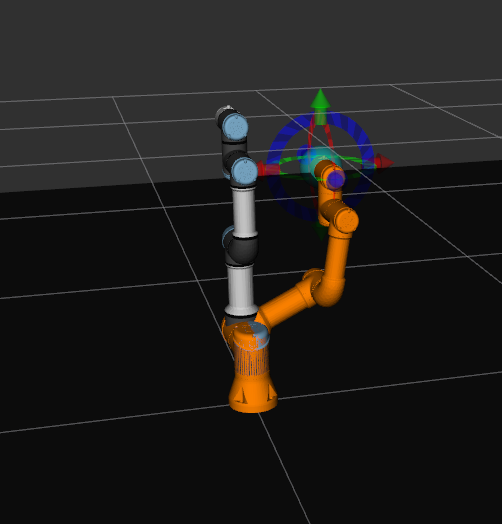
\includegraphics[width=\textwidth]{mover_extremo.png}
        \caption{Arrastre interactivo (\textit{Goal State}).}
        \label{fig:mover_extremo}
    \end{subfigure}
    \hfill
    \begin{subfigure}[b]{0.32\textwidth}
        \centering
        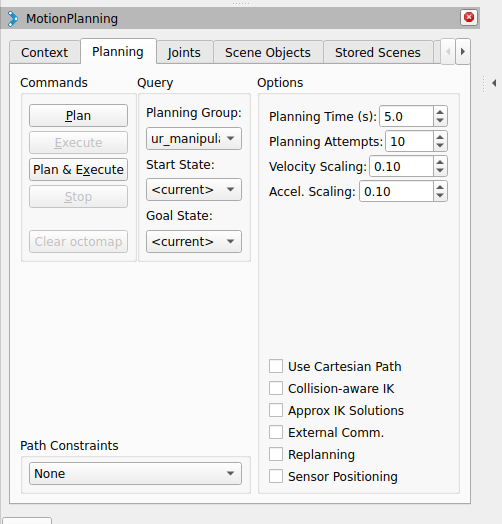
\includegraphics[width=\textwidth]{plan_and_execute.png}
        \caption{Panel \textit{MotionPlanning}.}
        \label{fig:panel_plan}
    \end{subfigure}
    \hfill
    \begin{subfigure}[b]{0.32\textwidth}
        \centering
        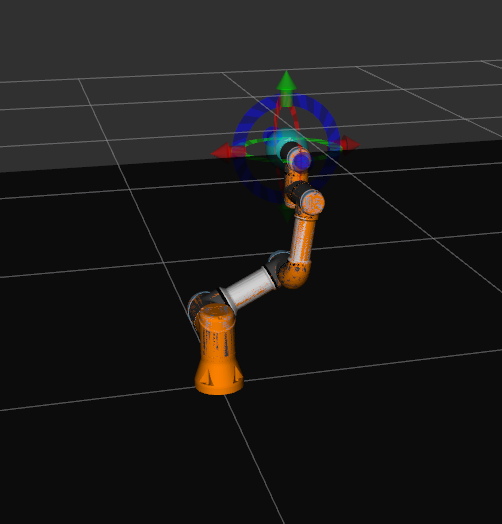
\includegraphics[width=\textwidth]{ejecutar.png}
        \caption{Trayectoria ejecutada con éxito.}
        \label{fig:ejecutar_exito}
    \end{subfigure}
    \caption{Secuencia de interacción manual en RViz2: fijación de meta cartesiana 3D mediante marcador interactivo, cálculo de trayectoria OMPL y ejecución dinámica en Gazebo.}
    \label{fig:grid_interaccion_manual}
\end{figure}

\subsection{Introspección del Middleware ROS 2 (Sección 6.1)}

Conforme a los requerimientos de la Sección 6.1 del guion, se procedió a interrogar al middleware utilizando herramientas CLI de introspección activa. Se detectaron \textbf{19 nodos funcionales} coordinando la simulación.

\subsubsection{Mapeo Detallado de Nodos e Interfaces}
La Tabla~\ref{tab:mapeo_interfaces_ur3e} resume las entradas, salidas, servicios y acciones de los nodos medulares del pipeline.

\begin{table}[htbp]
    \centering
    \footnotesize
    \begin{tabularx}{\textwidth}{>{\raggedright\arraybackslash}p{3.5cm} >{\raggedright\arraybackslash}p{3.4cm} >{\raggedright\arraybackslash}p{3.5cm} >{\raggedright\arraybackslash}X}
        \toprule
        \textbf{Nodo Activo} & \textbf{Tópicos Suscritos} & \textbf{Tópicos Publicados} & \textbf{Servicios / Acciones} \\
        \midrule
        \texttt{/move\_group} & \texttt{/joint\_states}, \texttt{/clock}, \texttt{/trajectory\_}\-\texttt{execution\_event} & \texttt{/display\_}\allowbreak\texttt{planned\_path}, \texttt{/monitored\_}\-\texttt{planning\_scene} & Acciones: \texttt{/move\_action}, \texttt{/execute\_trajectory}. \newline Srv: \texttt{/compute\_}\-\texttt{cartesian\_path} \\
        \addlinespace
        \texttt{/controller\_manager} & \texttt{/clock}, \texttt{/robot\_description} & \texttt{/controller\_}\allowbreak\texttt{manager/activity}, métricas de lazo & Srv: \texttt{/switch\_controller}, \texttt{/load\_controller} \\
        \addlinespace
        \texttt{/joint\_state\_}\-\texttt{broadcaster} & \texttt{/clock} & \texttt{/joint\_states}, \texttt{/dynamic\_joint\_states} & Srv: Parámetros del broadcaster \\
        \addlinespace
        \texttt{/scaled\_joint\_}\newline\texttt{trajectory\_controller} & \texttt{/clock}, consignas de trayectoria & \texttt{/controller\_state}, eventos de transición & Acción: \newline \texttt{/scaled\_joint\_}\allowbreak\texttt{trajectory\_}\allowbreak\texttt{controller/}\allowbreak\texttt{follow\_joint\_}\allowbreak\texttt{trajectory} \\
        \addlinespace
        \texttt{/robot\_state\_}\-\texttt{publisher} & \texttt{/joint\_states}, \texttt{/clock} & \texttt{/tf}, \texttt{/tf\_static}, \texttt{/robot\_description} & Srv: Introspección URDF \\
        \addlinespace
        \texttt{/rviz2\_moveit} & \texttt{/display\_}\allowbreak\texttt{planned\_path}, \texttt{/tf}, \texttt{/tf\_static} & Feedback de marcadores, \texttt{/goal\_pose} & Cliente de acción: \texttt{/move\_action} \\
        \bottomrule
    \end{tabularx}
    \caption{Mapeo de interfaces de los componentes principales del Bloque 4.}
    \label{tab:mapeo_interfaces_ur3e}
\end{table}

\subsubsection{Grafo Computacional Dinámico (\texttt{rqt\_graph})}
El análisis gráfico ejecutado con \texttt{ros2 run rqt\_graph rqt\_graph} (Figura~\ref{fig:grafo_nodos}) confirma la arquitectura desacoplada: \texttt{joint\_state\_broadcaster} actúa como el puente sensorial alimentando a \texttt{robot\_state\_publisher} y a \texttt{move\_group}, mientras que la ejecución de comandos se delega al controlador articular de \texttt{ros2\_control}.

\begin{figure}[htbp]
    \centering
    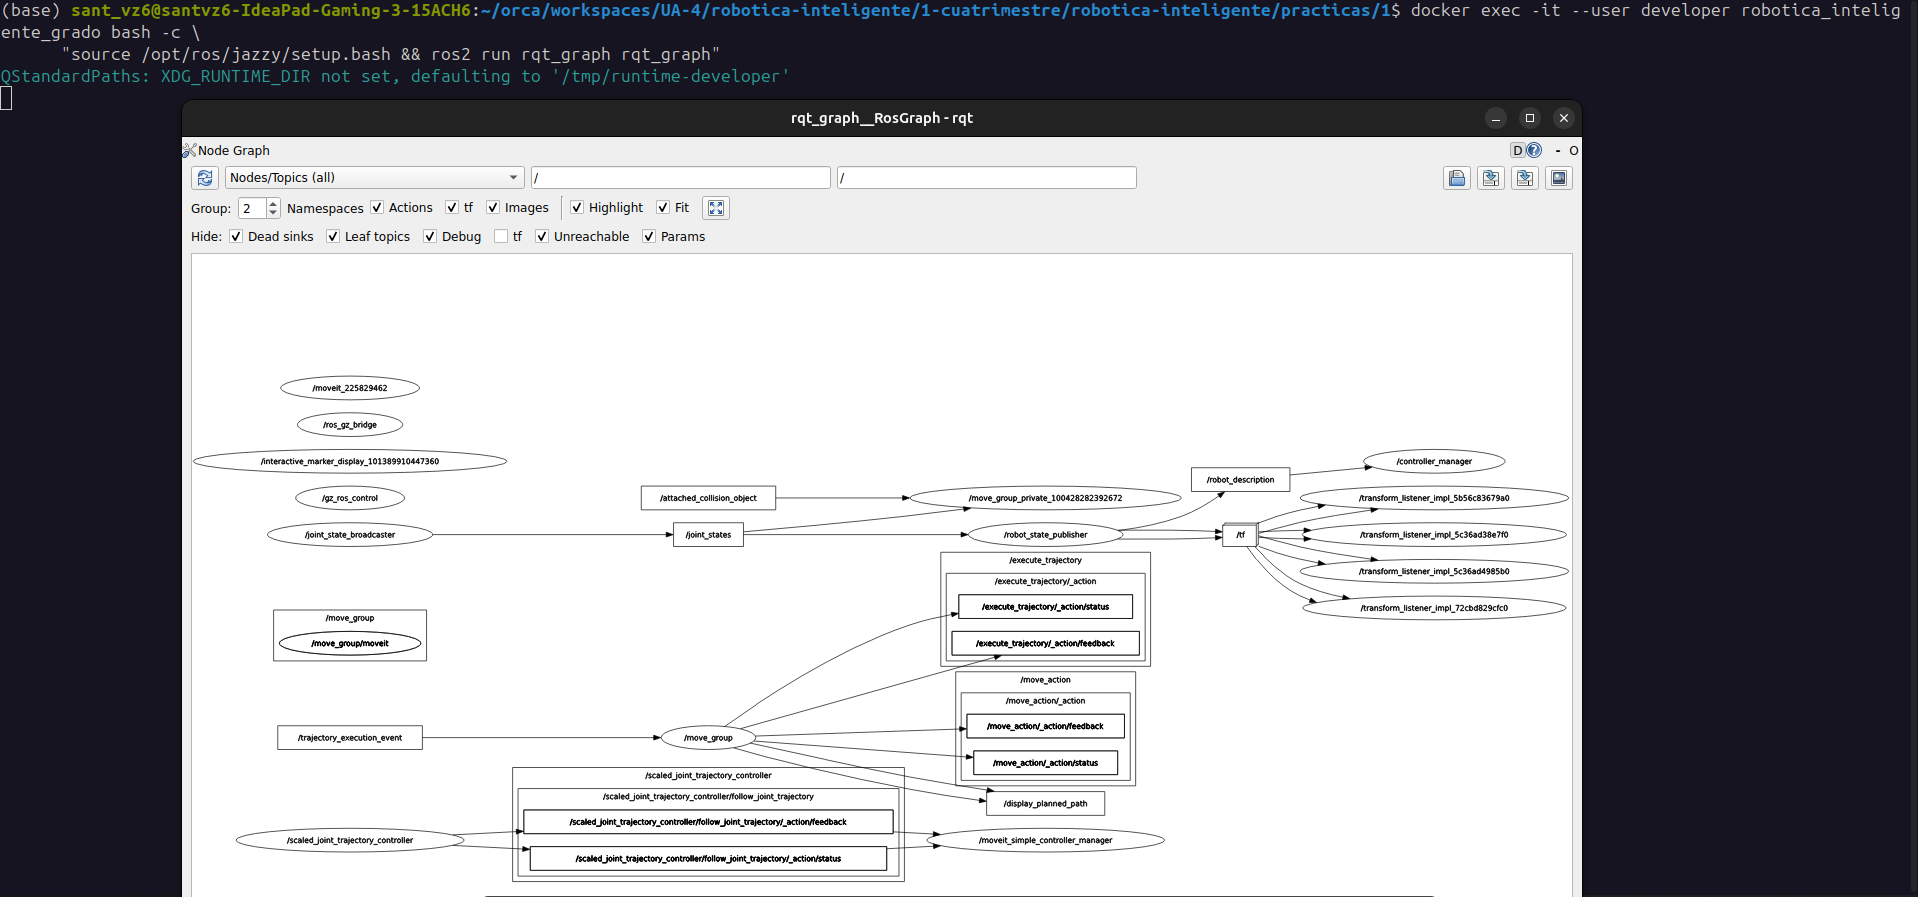
\includegraphics[width=0.95\textwidth]{grafo_nodos.png}
    \caption{Grafo dinámico de nodos y tópicos del sistema capturado en vivo mediante \texttt{rqt\_graph}.}
    \label{fig:grafo_nodos}
\end{figure}

\subsection{Explicación del Flujo de Información y Cinemática}

Para comprender cómo funciona el sistema en conjunto, analizamos el recorrido de la información desde que solicitamos una postura hasta que el robot se mueve en el simulador:

\begin{enumerate}
    \item \textbf{Definición de la meta (Pose objetivo):}\\
    Se indica la posición $(X, Y, Z)$ y la orientación deseada para el extremo del robot (\texttt{tool0}). Esta orden puede enviarse de forma manual arrastrando el marcador 3D en RViz2 o mediante comandos desde la terminal utilizando el script en Python.

    \item \textbf{Cálculo de cinemática inversa y planificación (MoveIt 2):}\\
    El nodo \texttt{move\_group} procesa la petición realizando dos pasos fundamentales:
    \begin{itemize}
        \item \textbf{Cinemática inversa (IK):} Calcula los ángulos necesarios en cada una de las 6 articulaciones del brazo ($\theta_1, \dots, \theta_6$) para situar el extremo en la coordenada espacial solicitada.
        \item \textbf{Planificación de trayectoria:} Con los ángulos objetivo, el planificador (OMPL) busca un camino libre de colisiones entre la postura actual y la meta, generando una secuencia de puntos suave que respeta los límites de velocidad y aceleración del brazo.
    \end{itemize}

    \item \textbf{Ejecución del movimiento (\texttt{ros2\_control}):}\\
    Una vez calculada la trayectoria, MoveIt la transmite al controlador articular de trayectoria mediante la acción de ROS 2 \texttt{FollowJointTrajectory}. El nodo \texttt{scaled\_joint\_}\-\texttt{trajectory\_controller} guía a los motores para recorrer la ruta en el tiempo previsto.

    \item \textbf{Simulación física y realimentación sensorial (Gazebo y TF2):}\\
    Gazebo aplica el movimiento a las articulaciones físicas del robot en el entorno virtual. En paralelo, los sensores del simulador leen la posición real de cada articulación y la publican en el tópico \texttt{/joint\_states}. A partir de estas lecturas, el nodo \texttt{robot\_state\_publisher} actualiza el árbol de transformaciones geométricas (\texttt{/tf}), permitiendo que RViz2 refleje en tiempo real la postura exacta del robot.
\end{enumerate}

\subsection{Análisis e Interpretación del Árbol de Transformaciones (TF2)}

La comprensión espacial de la cadena cinemática se verificó mediante la herramienta \texttt{ros2 run tf2\_tools view\_frames} (Figura~\ref{fig:grid_tf}).

\begin{figure}[htbp]
    \centering
    \begin{subfigure}[b]{0.48\textwidth}
        \centering
        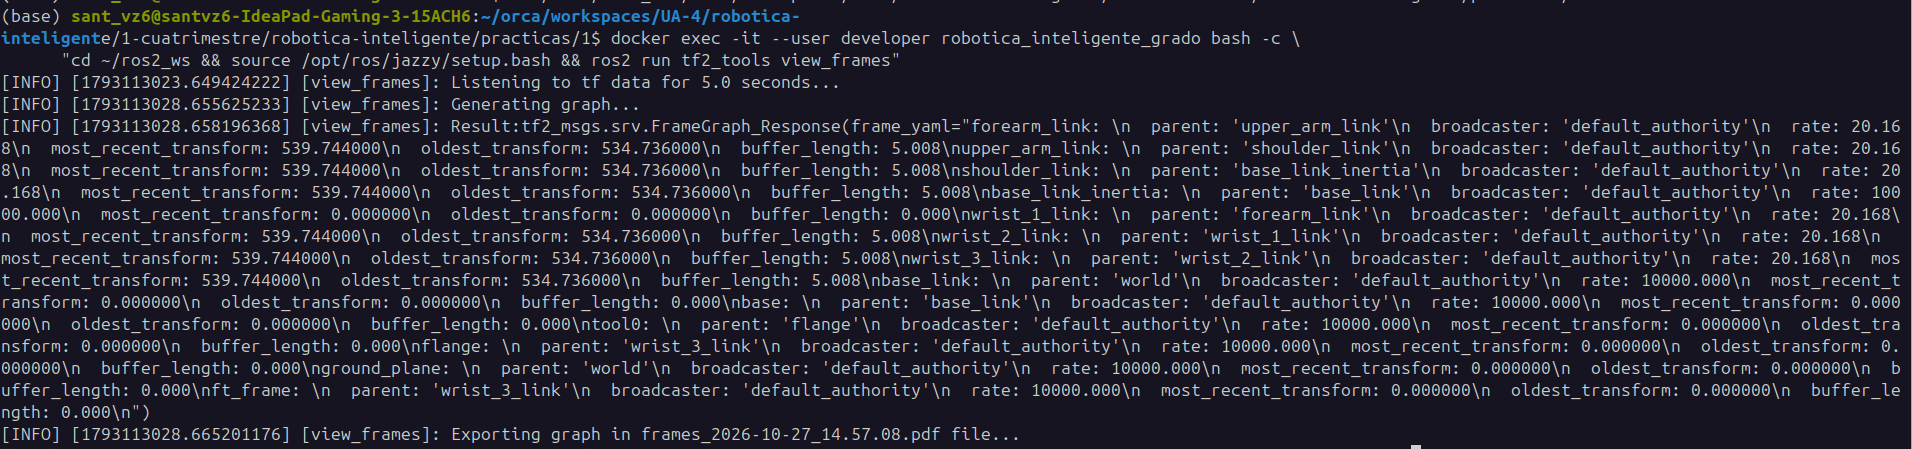
\includegraphics[width=\textwidth]{arbol-tf2.png}
        \caption{Extracción de \textit{frames} con \texttt{view\_frames}.}
        \label{fig:tf_view_frames}
    \end{subfigure}
    \hfill
    \begin{subfigure}[b]{0.48\textwidth}
        \centering
        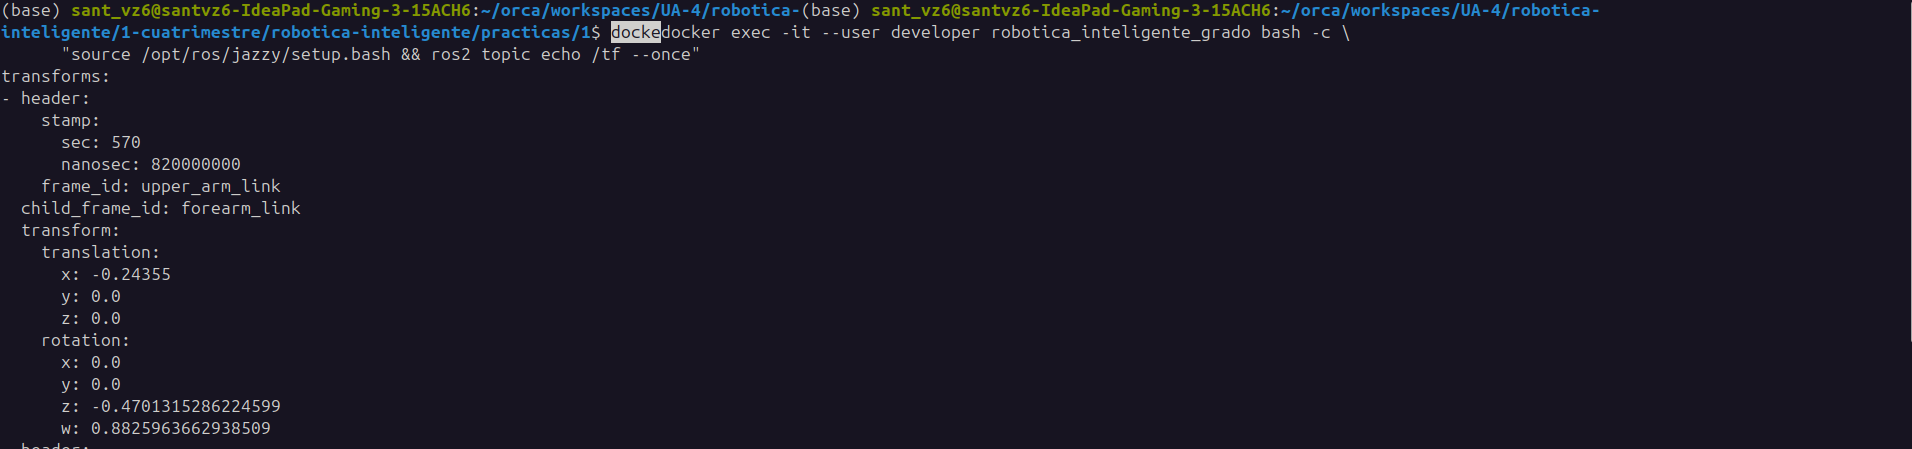
\includegraphics[width=\textwidth]{transformacion_dinamica.png}
        \caption{Inspección en vivo con \texttt{echo /tf --once}.}
        \label{fig:tf_echo}
    \end{subfigure}
    \caption{Introspección del árbol espacial de transformaciones geométricas (TF2) en consola.}
    \label{fig:grid_tf}
\end{figure}

El árbol jerárquico se compone de \textbf{14 marcos de referencia} encadenados:
\begin{align*}
    \text{world} &\longrightarrow \text{base\_link} \longrightarrow \text{base\_link\_inertia} \longrightarrow \text{shoulder\_link} \longrightarrow \text{upper\_arm\_link} \\
    &\longrightarrow \text{forearm\_link} \longrightarrow \text{wrist\_1\_link} \longrightarrow \text{wrist\_2\_link} \longrightarrow \text{wrist\_3\_link} \longrightarrow \text{flange} \longrightarrow \text{tool0}
\end{align*}

\begin{itemize}
    \item \textbf{Transformaciones Estáticas (\texttt{/tf\_static}):} Invariantes en el tiempo, tales como la fijación del robot al suelo (\texttt{world -> base\_link}), la inercia interna de la peana y la distancia fija entre la brida mecánica y el centro de herramienta (\texttt{flange -> tool0}).
    \item \textbf{Transformaciones Dinámicas (\texttt{/tf}):} Publicadas a una frecuencia nominal de \textbf{20.16 Hz} por \texttt{robot\_state\_publisher}. Cada enlace móvil transmite un vector de traslación constante (longitud del eslabón) y un cuaternión de rotación unitario variable que refleja en tiempo real el ángulo del servomotor.
\end{itemize}

\subsection{Tarea de Programación Opcional: Control en Python (Sección 6.2)}

Para aspirar a la máxima calificación según la Sección 6.2 del guion, se programó y validó el script en Python \texttt{ur3e\_send\_pose.py} en el espacio de trabajo persistente (\texttt{\textasciitilde/ros2\_ws/p1\_scripts/}). Este script prescinde enteramente de la interfaz gráfica RViz2, conectándose como cliente directo a las acciones de ROS 2.

Se validaron tres modos de control en la consola (Figura~\ref{fig:grid_pruebas_python}):

\begin{enumerate}
    \item \textbf{Prueba A -- Modo Articular Directo (\texttt{--mode joint}):}\\
    Envío directo de la configuración articular $\boldsymbol{\theta} = [0.0, -1.57, 1.57, -1.57, -1.57, 0.0]\,\text{rad}$ al nodo \texttt{scaled\_joint\_}\-\texttt{trajectory\_controller}. El manipulador flexiona el codo en ángulo recto con perfil suave interpolado en 4.0 segundos.
    \begin{lstlisting}[language=bash]
python3 ur3e_send_pose.py --mode joint --joints 0.0 -1.57 1.57 -1.57 -1.57 0.0
    \end{lstlisting}

    \item \textbf{Prueba B -- Modo Cinemático Cartesiano 3D (\texttt{--mode cartesian}):}
    Fijación de coordenada espacial $(X=0.25\,\text{m}, Y=0.15\,\text{m}, Z=0.35\,\text{m})$ con orientación vertical ($\mathrm{pitch}=\pi$). La orden viaja al servidor de acción \texttt{/move\_action} de MoveIt 2, el cual calcula cinemática inversa y trayectoria OMPL sin colisiones antes de ejecutar.
    \begin{lstlisting}[language=bash]
python3 ur3e_send_pose.py --mode cartesian --x 0.25 --y 0.15 --z 0.35
    \end{lstlisting}

    \item \textbf{Prueba C -- Poses Semánticas SRDF (\texttt{--mode named}):}
    Carga de posturas preestablecidas de fábrica (\texttt{home}, \texttt{up}, \texttt{test\_configuration}) definidas en el archivo semántico SRDF de Universal Robots.
    \begin{lstlisting}[language=bash]
python3 ur3e_send_pose.py --mode named --named home
    \end{lstlisting}
\end{enumerate}

\begin{figure}[htbp]
    \centering
    \begin{subfigure}[b]{0.32\textwidth}
        \centering
        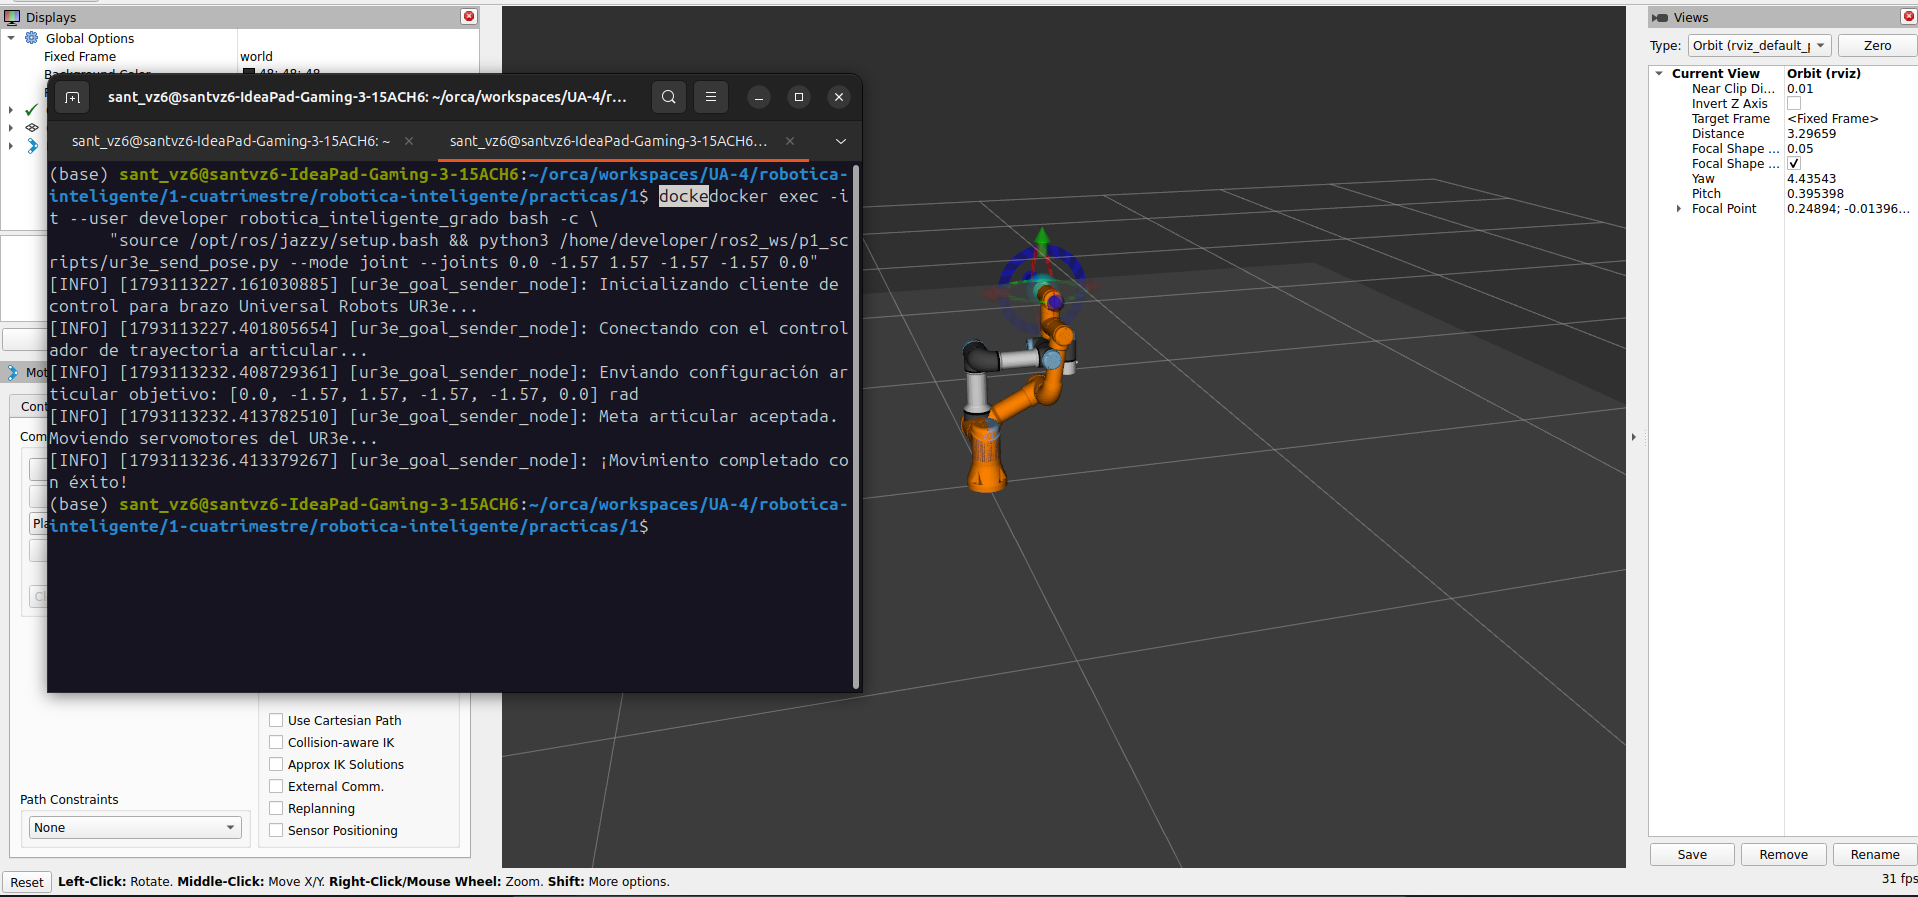
\includegraphics[width=\textwidth]{prueba-A_control_directo.png}
        \caption{Prueba A: Control Articular.}
        \label{fig:prueba_a}
    \end{subfigure}
    \hfill
    \begin{subfigure}[b]{0.32\textwidth}
        \centering
        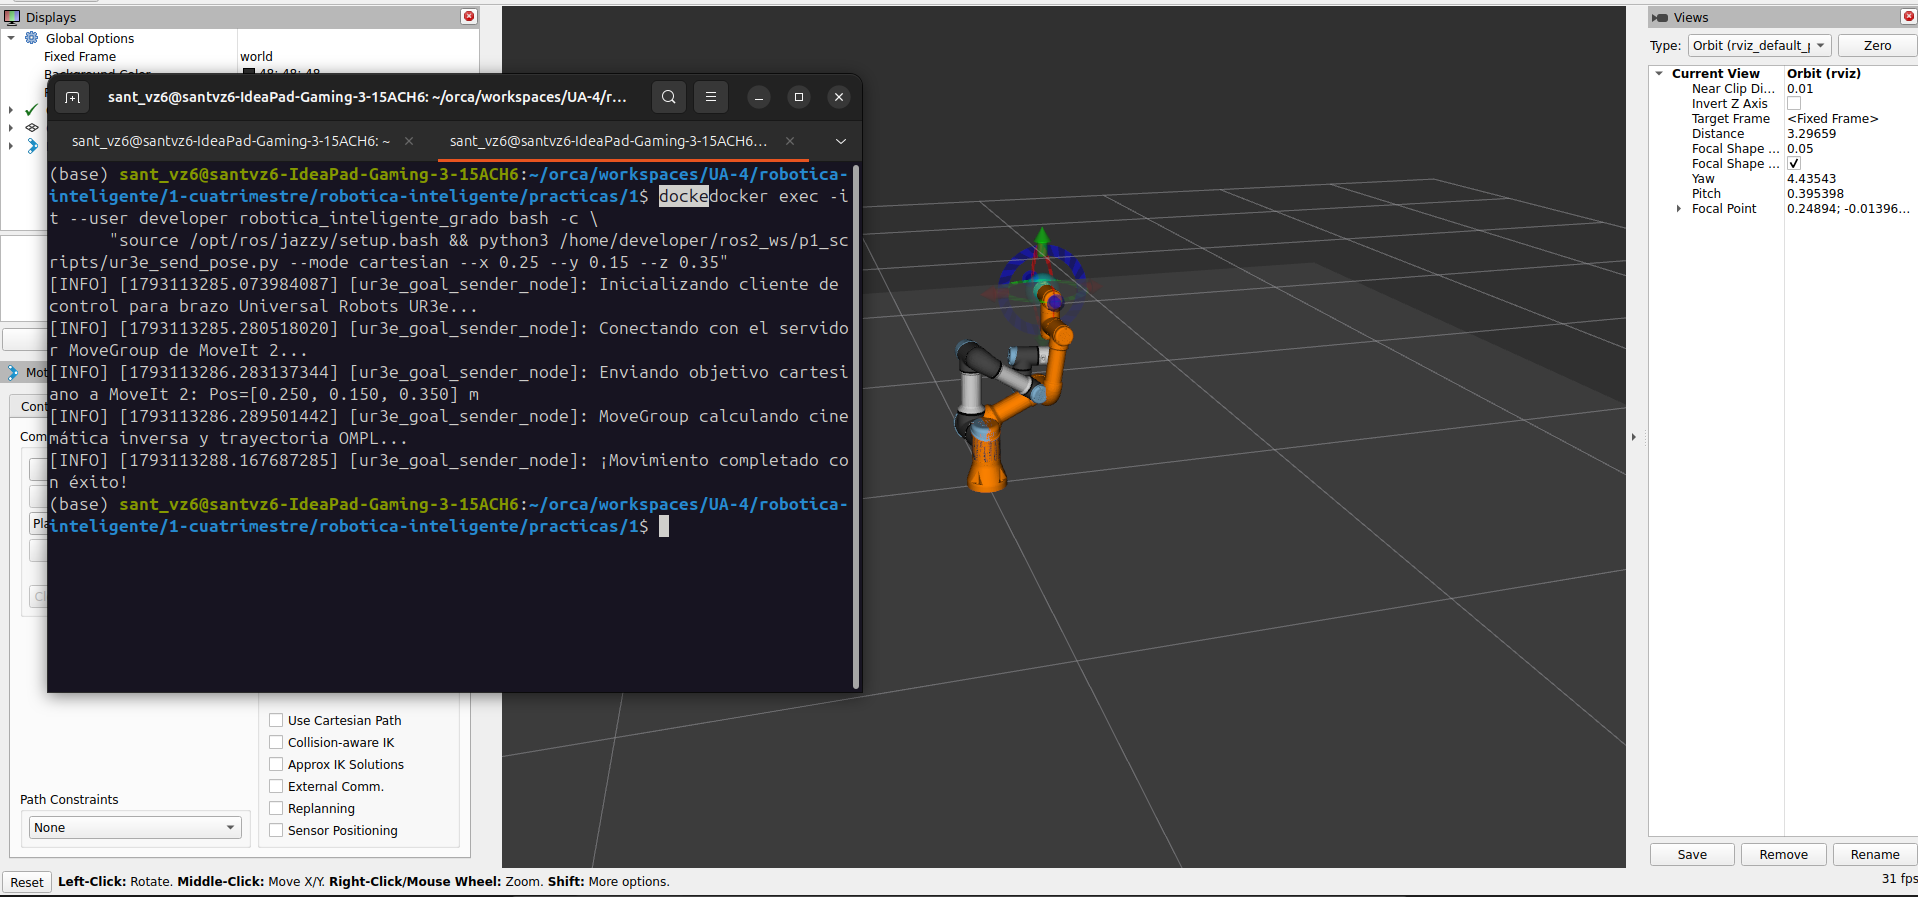
\includegraphics[width=\textwidth]{prueba-B_control_cartesiano_3d.png}
        \caption{Prueba B: Meta Cartesiana 3D.}
        \label{fig:prueba_b}
    \end{subfigure}
    \hfill
    \begin{subfigure}[b]{0.32\textwidth}
        \centering
        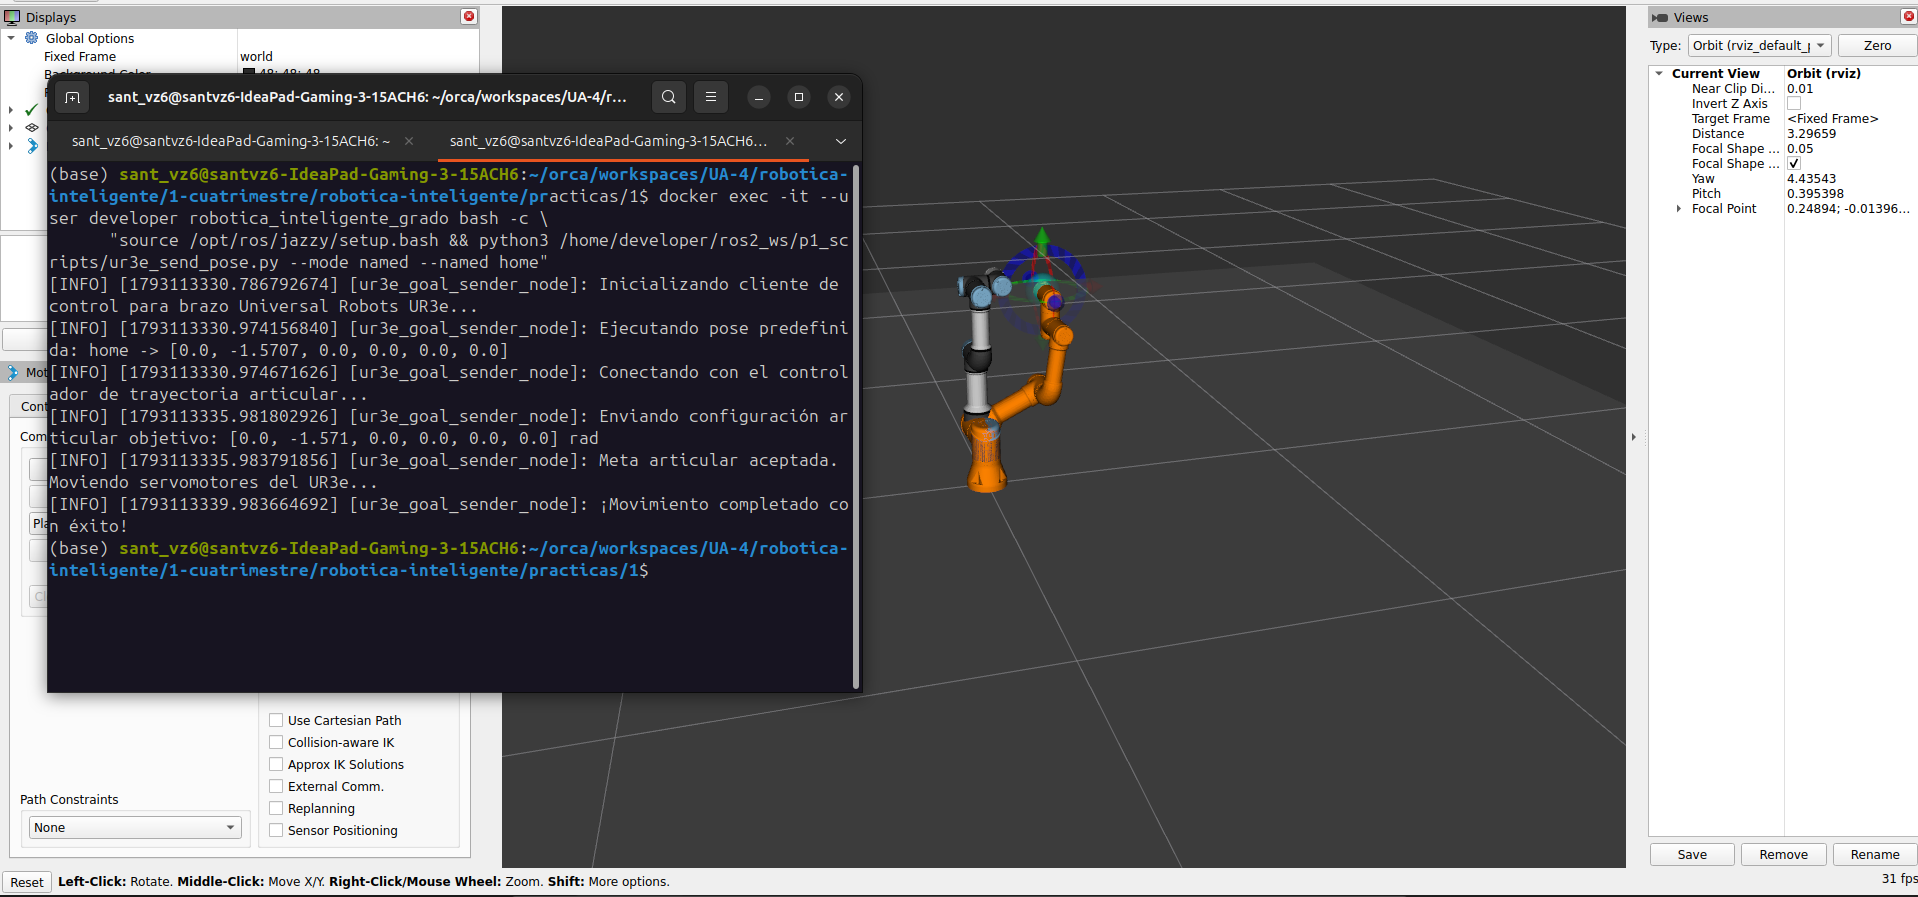
\includegraphics[width=\textwidth]{prueba-C_poses_sematicas_srdf.png}
        \caption{Prueba C: Pose Semántica \textit{home}.}
        \label{fig:prueba_c}
    \end{subfigure}
    \caption{Validación experimental de la tarea de programación opcional (Sección 6.2): ejecución de comandos desde la terminal y respuesta síncrona del robot en RViz2 y Gazebo.}
    \label{fig:grid_pruebas_python}
\end{figure}

\end{document}
